\documentclass[10pt,draftclsnofoot,onecolumn,letterpaper,compsoc]{IEEEtran}

\usepackage[margin=0.75in]{geometry}
\usepackage{float}
\usepackage{graphicx}
\usepackage{caption}
\usepackage{hyperref}
\usepackage{enumerate}
\usepackage{tabu}
\usepackage[english]{babel}\usepackage[numbers]{natbib}
\usepackage{natbib}
\usepackage{longtable}
\usepackage{vhistory}
\usepackage{pgfgantt}
\usepackage{listings}
\usepackage{color}
\usepackage{pdfpages}
\usepackage{lscape}

\definecolor{codegreen}{rgb}{0,0.6,0}
\definecolor{codegray}{rgb}{0.5,0.5,0.5}
\definecolor{codepurple}{rgb}{0.58,0,0.82}
\definecolor{backcolour}{rgb}{0.95,0.95,0.92}

\lstdefinestyle{mystyle}{
	backgroundcolor=\color{backcolour},   
	commentstyle=\color{codegreen},
	keywordstyle=\color{magenta},
	numberstyle=\tiny\color{codegray},
	stringstyle=\color{codepurple},
	basicstyle=\footnotesize,
	breakatwhitespace=false,         
	breaklines=true,                 
	captionpos=b,                    
	keepspaces=true,                 
	numbers=left,                    
	numbersep=5pt,                  
	showspaces=false,                
	showstringspaces=false,
	showtabs=false,                  
	tabsize=2
}
\lstset{style=mystyle}
\renewcommand{\linespread}{1.0}
\renewcommand{\bibsection}{}

\lstset{
captionpos=b,           
}
\title{Prototype Big Data Archive in a Public Cloud}
\author{
  \IEEEauthorblockN{Group 56: Pathfinder of Big Data\\Zhi Jiang, Isaac T Chan, Zhaoheng Wang} \\
  \IEEEauthorblockA{CS 463: Senior Capstone Spring 2017 \\ Oregon State University}
}
\date{}

\IEEEtitleabstractindextext{
	\begin{abstract}
	OSU campuses generate data constantly from multiples sources, including computer labs, wireless usage, student devices, and many others. This quantity of data, also known as big data, can effectively represent all kinds of behaviors of students for information technology. Currently, the data is very difficult to manage because it is collected from multiple sources and is impossible to analyze. Therefore, this project requires the use of various technologies for support. There are nine pieces of technologies required:1) Methods to measure performance metrics of database functionality. 2) Methods of database security. 3) Methods of user interaction with the system. 4) The framework and storage of processing unprocessed data 5) The ingestion and parsing for unprocessed data.  6) The operation for formatted and cleaned data in data storage 7) The storage way for dealing with processed data. 8) The programming language for achieving database functionality. 9) The visualization tool use to display the data. For each piece, we will provide the best three technology options. Our goal for this paper is to analyze each technology option and determine the optimal technology that we will implement.
\end{abstract}
}

\begin{document}
% cover page    
    \maketitle
    \IEEEdisplaynontitleabstractindextext
    \IEEEpeerreviewmaketitle
    \newpage

% catalog    
    \tableofcontents
	%\resizebox{\textwidth}{!}
    \newpage

% content   
	\section{Introduction}
	\subsection{Purpose}
    OSU campuses generate data constantly from multiples sources, including computer labs, wireless usage, student devices, and many others. This quantity of data, also known as big data, can effectively represent student behaviors for information technology. For example, analysis can be run to determine common student behaviors in order to allocate OSU resources to more often used utilities. Currently, the data is very difficult to manage because it is collected from multiple sources and is impossible to analyze. The data is neither stored in the same formats nor in the same locations, meaning it is inaccessible and useful information is unable to be extracted. The purpose of this project is to unify the data onto the consistent cloud platform of Amazon Web Services, which additionally provides utilities to manage and analyze.
    
    \subsection{Current Position}
    Currently, the functional part of the project is complete. We have a working database implementation in the Amazon Web Services public cloud, with appropriate storage, loading, and restricted access for sensitive data. By leveraging additional services in the AWS environment, we are able to provide rudimentary analysis, reporting, and visualization of data. From this position, we are able to present at Expo on the entire project, from beginning to end, including potential outcomes if the project were adopted by OSU. In the original project description, there were three deliverables listed. We have completed two of them: the database implementation and analysis/reporting/visualization. The third, a cost model, has yet to be complete. In order to provide an accurate cost model, we require an estimate for data amounts and are currently waiting for the estimate. This deliverable won't affect the project demonstration at Expo and is soley for the benefit of our client to decide on whether OSU will adopt our prototype.
    \newpage
    \section{Requirements}
	\subsection{Original Document}
	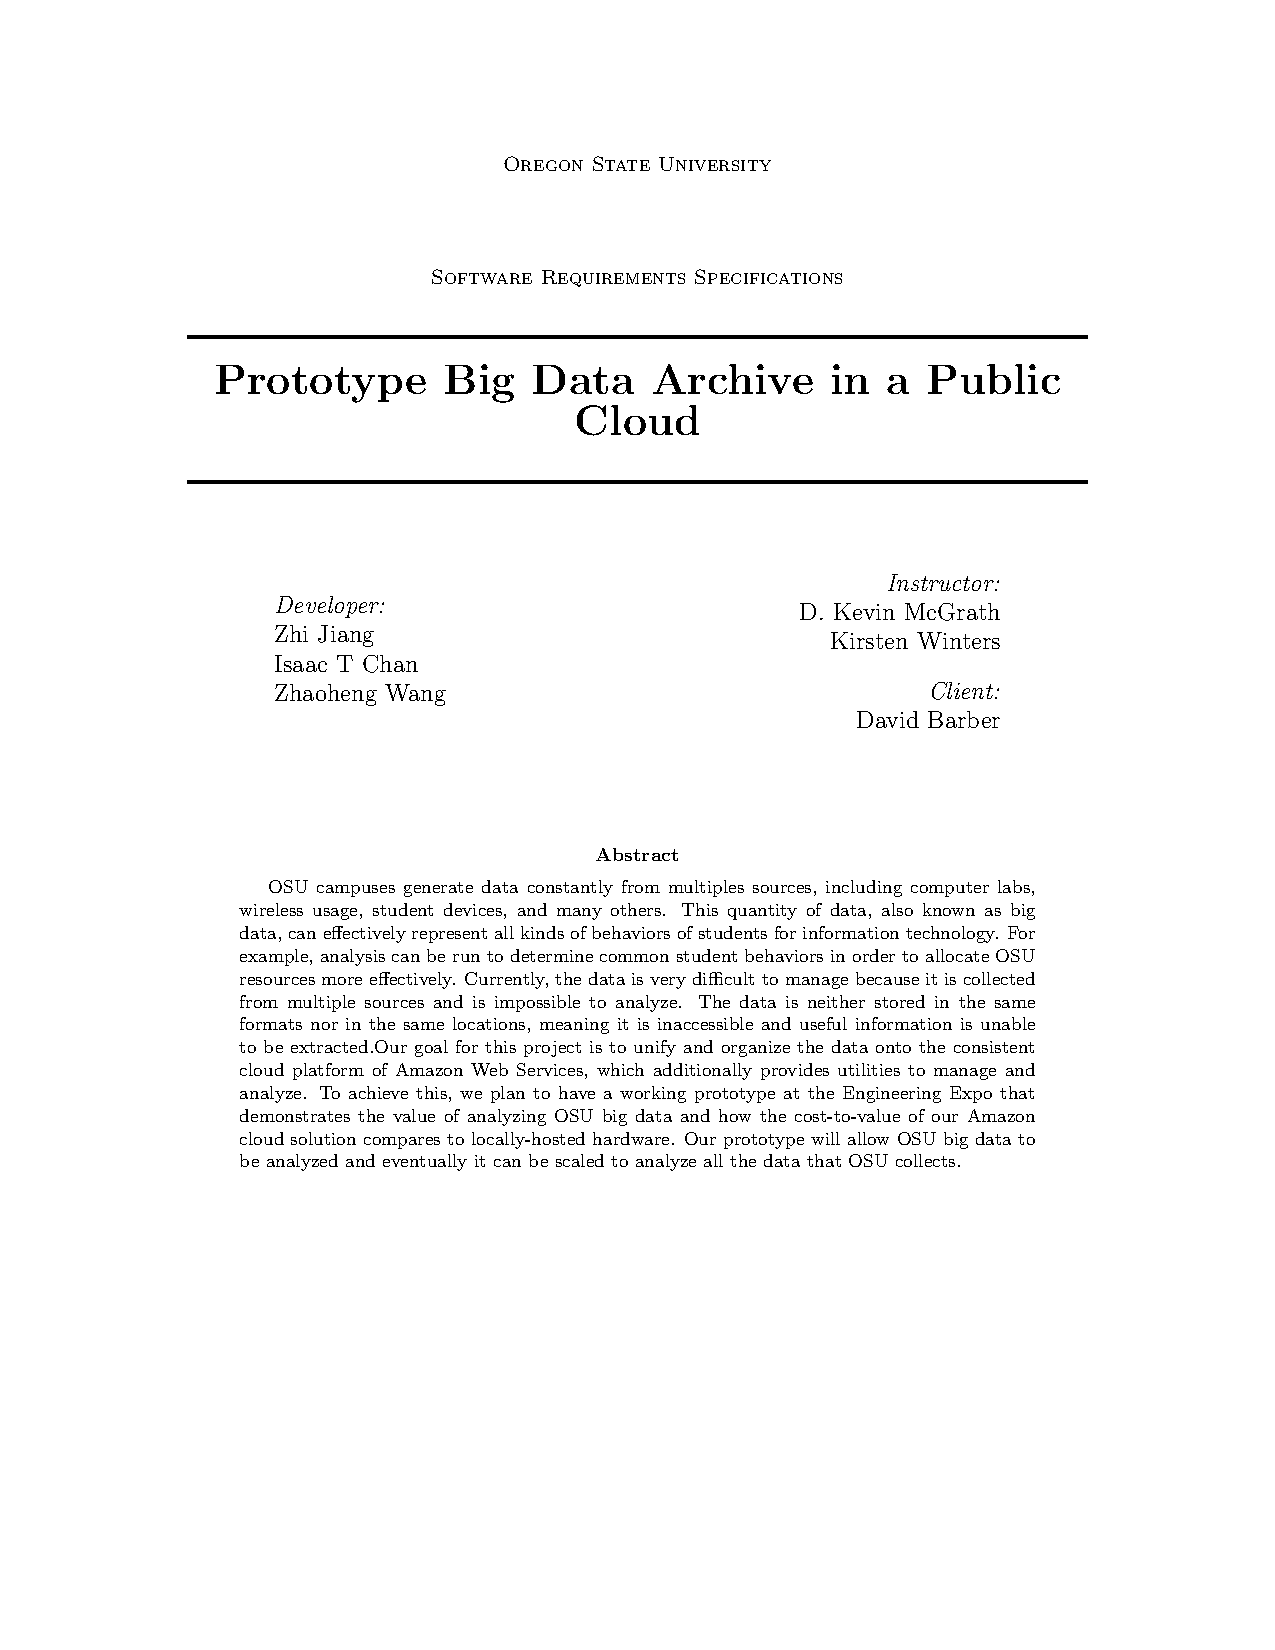
\includepdf[pages=-]{Original_Doc/original_requirements.pdf}
    \subsection{Requirements Revision}
\vspace*{+30pt}
\begin{tabular}{| p{0.01\linewidth} | p{0.4\linewidth} | p{0.1\linewidth} | p{0.40\linewidth} |}\hline
1 & The user can insert any types of data they want into database & Changed & The user cannot insert data into database directly, all data are imported by script from data storage to database.\\ 
\hline
2 & Create table in database & Added & In order to achieve better automation, we use script to create table when we import data.\\ 
\hline
3 & Import data from data storage to database & Added & All data are stored in data storage at the beginning, and then we use script to import them into database.\\ 
\hline
4 & Data anonymization & Added & This is a new requirement of client. We separate Mac address, ONID and the rest of data into three different table in database.\\ 
\hline
5 & Data Visualization & Added &  According to the requirements from our client, we need to do the rudimentary analysis on visualization tool\\ 
\hline
6 & Database Performance & Changed &  Due to the small volume of data ingestion, this requirement had reduced priority.\\ 
\hline
7 & Tests for Functionality & Changed &  Instead of testing for viability of analysis, our client requested a data standardization step, which was run on data that would be loaded into the database.\\ 
\hline
\end{tabular}

    \newpage
    \begin{landscape}
\subsection{The Entire Process}
	\vspace*{+30pt}
	\begin{ganttchart}[y unit chart=0.7cm, vgrid, hgrid]{1}{31}
     	\gantttitle{Fall}{9}
        \gantttitle{Winter}{11}
        \gantttitle{Spring}{11}\\
       
        \gantttitlelist{3,...,11}{1}
        \gantttitlelist{1,...,11}{1}
        \gantttitlelist{1,...,11}{1}\\
        
        % Fall start 1 to 9
        \ganttbar{Requirements Document}{1}{3}\\
        \ganttbar{Technology Review}{4}{6} \\
        \ganttbar{Design Document}{7}{8} \\
        \ganttbar{Progress Report}{9}{9}\\
        
        % Winter start 10 to 20
        \ganttbar{Creating EC2}{10}{12}\\
        \ganttbar{Creating table by script}{13}{15}\\
        \ganttbar{Importing data by script}{13}{15}\\
        \ganttbar{Data visualization on QuickSight}{15}{16}\\
        \ganttbar{Winter Term Midterm Progress Report}{16}{17}\\
        \ganttbar{Changing table structure}{17}{18} \\
        \ganttbar{Adding workflow of loading new data }{17}{18}\\
        \ganttbar{Updating data in DynamoDB table}{18}{19}\\
        \ganttbar{Winter Term Progress Report}{19}{20}\\
        
        % Spring start 21 to 31
        %\ganttbar{Test for functionality}{}{} \\
        %\ganttbar{Performance Optimization}{}{}\\
        %\ganttbar{Security Optimization}{}{}\\
        %\ganttbar{Cost Comparison}{}{}\\
        \ganttbar{Tests for Feasibility}{21}{23}\\
        \ganttbar{Cost Analysis}{23}{24}\\
        \ganttbar{Spring Term Midterm Progress Report}{25}{27}\\
        \ganttbar{Expo}{27}{27}\\
        \ganttbar{Client Demo}{28}{28}\\
        \ganttbar{Anonymization Function}{28}{28}\\
        \ganttbar{Final Report}{29}{31}
	\end{ganttchart}
\end{landscape}
    \newpage
    \section{Technology Review}
	\subsection{Original Document}
    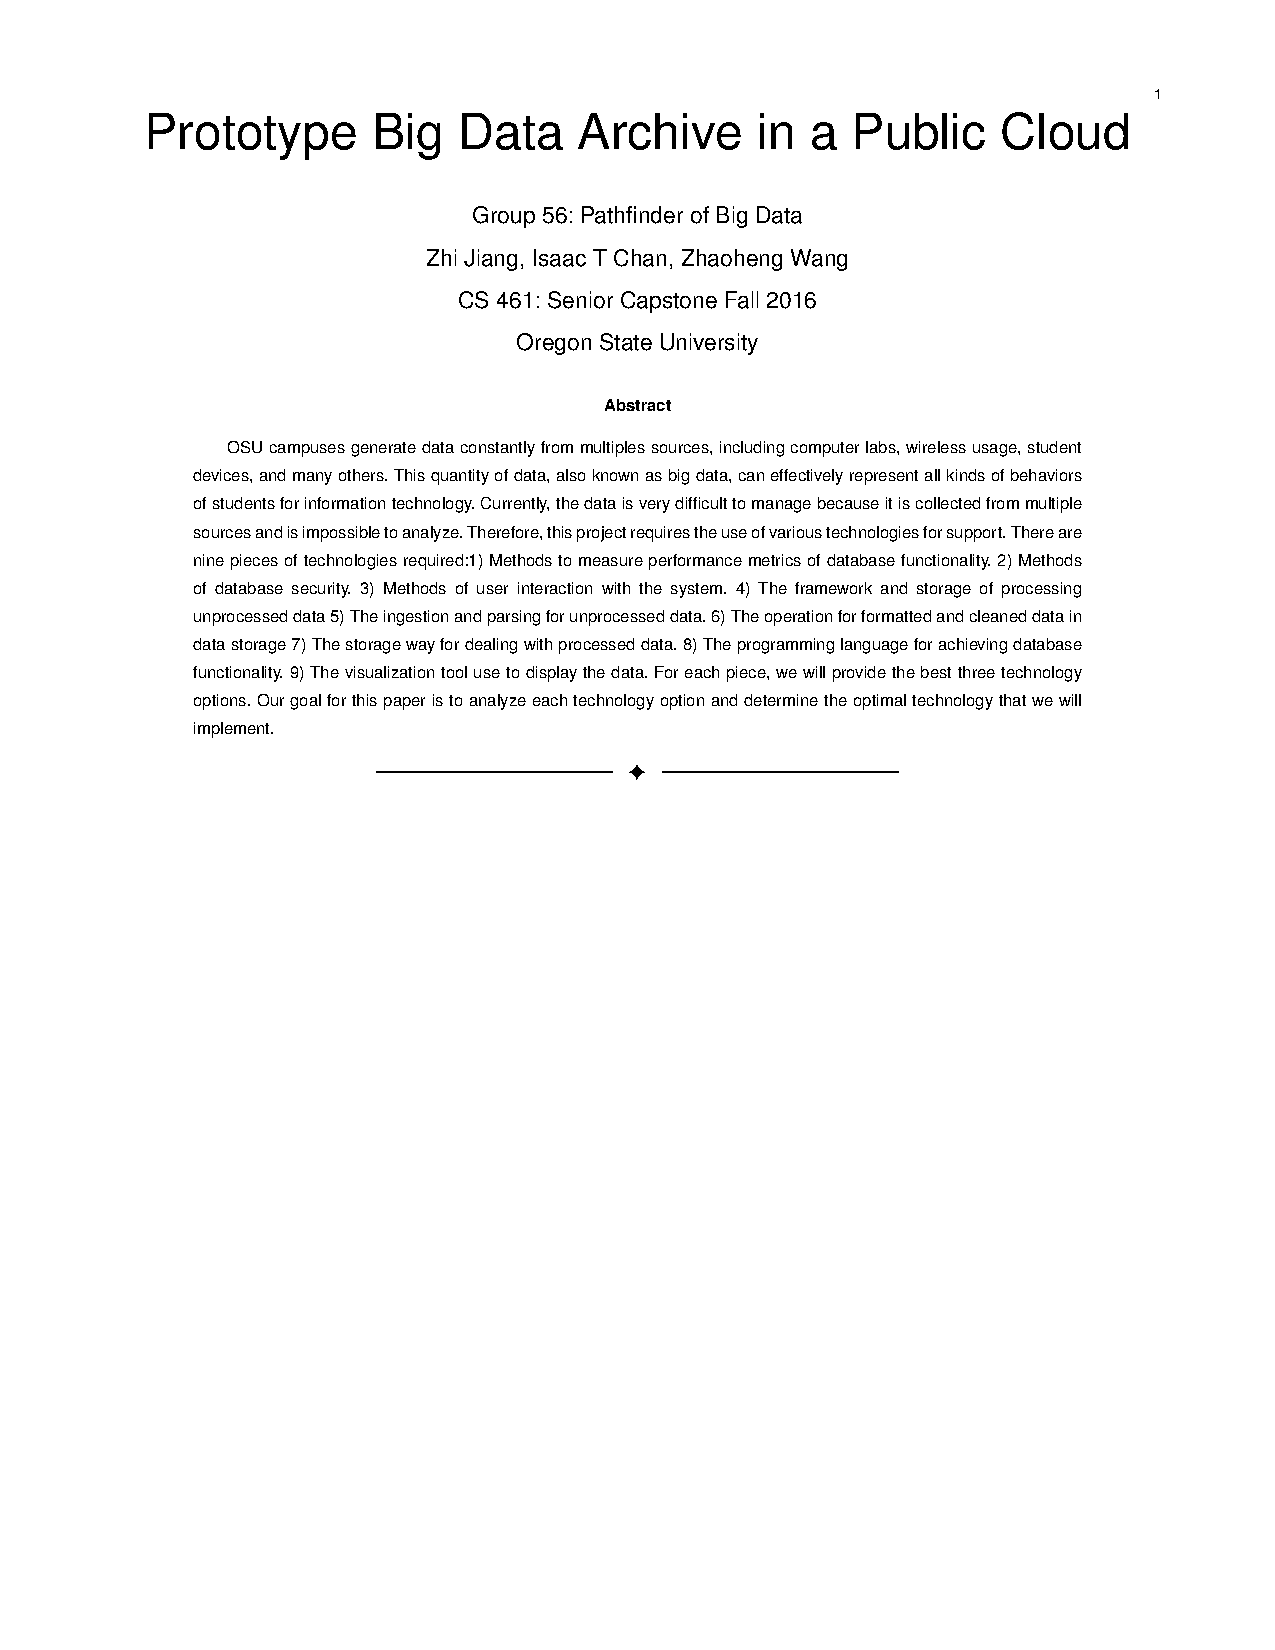
\includepdf[pages=-]{Original_Doc/original_technology.pdf}
	\subsection{Technology Review Revision}
\noindent In our technology review document, we would like to some tools for ingestion and parsing of unprocessed data such as Apache Spark and Amazon Kinesis, but eventually, we did not use them. The reason is in fact; we are not required to complete ingestion and parsing of data. The client has provided existing data. Thus we do not need to consider how to ingest data by ourselves.\\

\noindent We change the language for implementing database table. Instead of using Java APIs, we are using the Python SDK for implementing DynamoDB table. The reason is Java APIs only show how to implement the DynamoDB table but they don't have the steps for loading data from S3 to DynamoDB. In boto3, We find the specific steps for loading data from S3 to DynamoDB through EC2 instances. Furthermore, it is better to use the same language for loading data and implementing DynamoDB table. Therefore, we decide to use the Python language to do the implementation.\\
         
    \newpage
    \section{Design}
	\subsection{Original Document}
    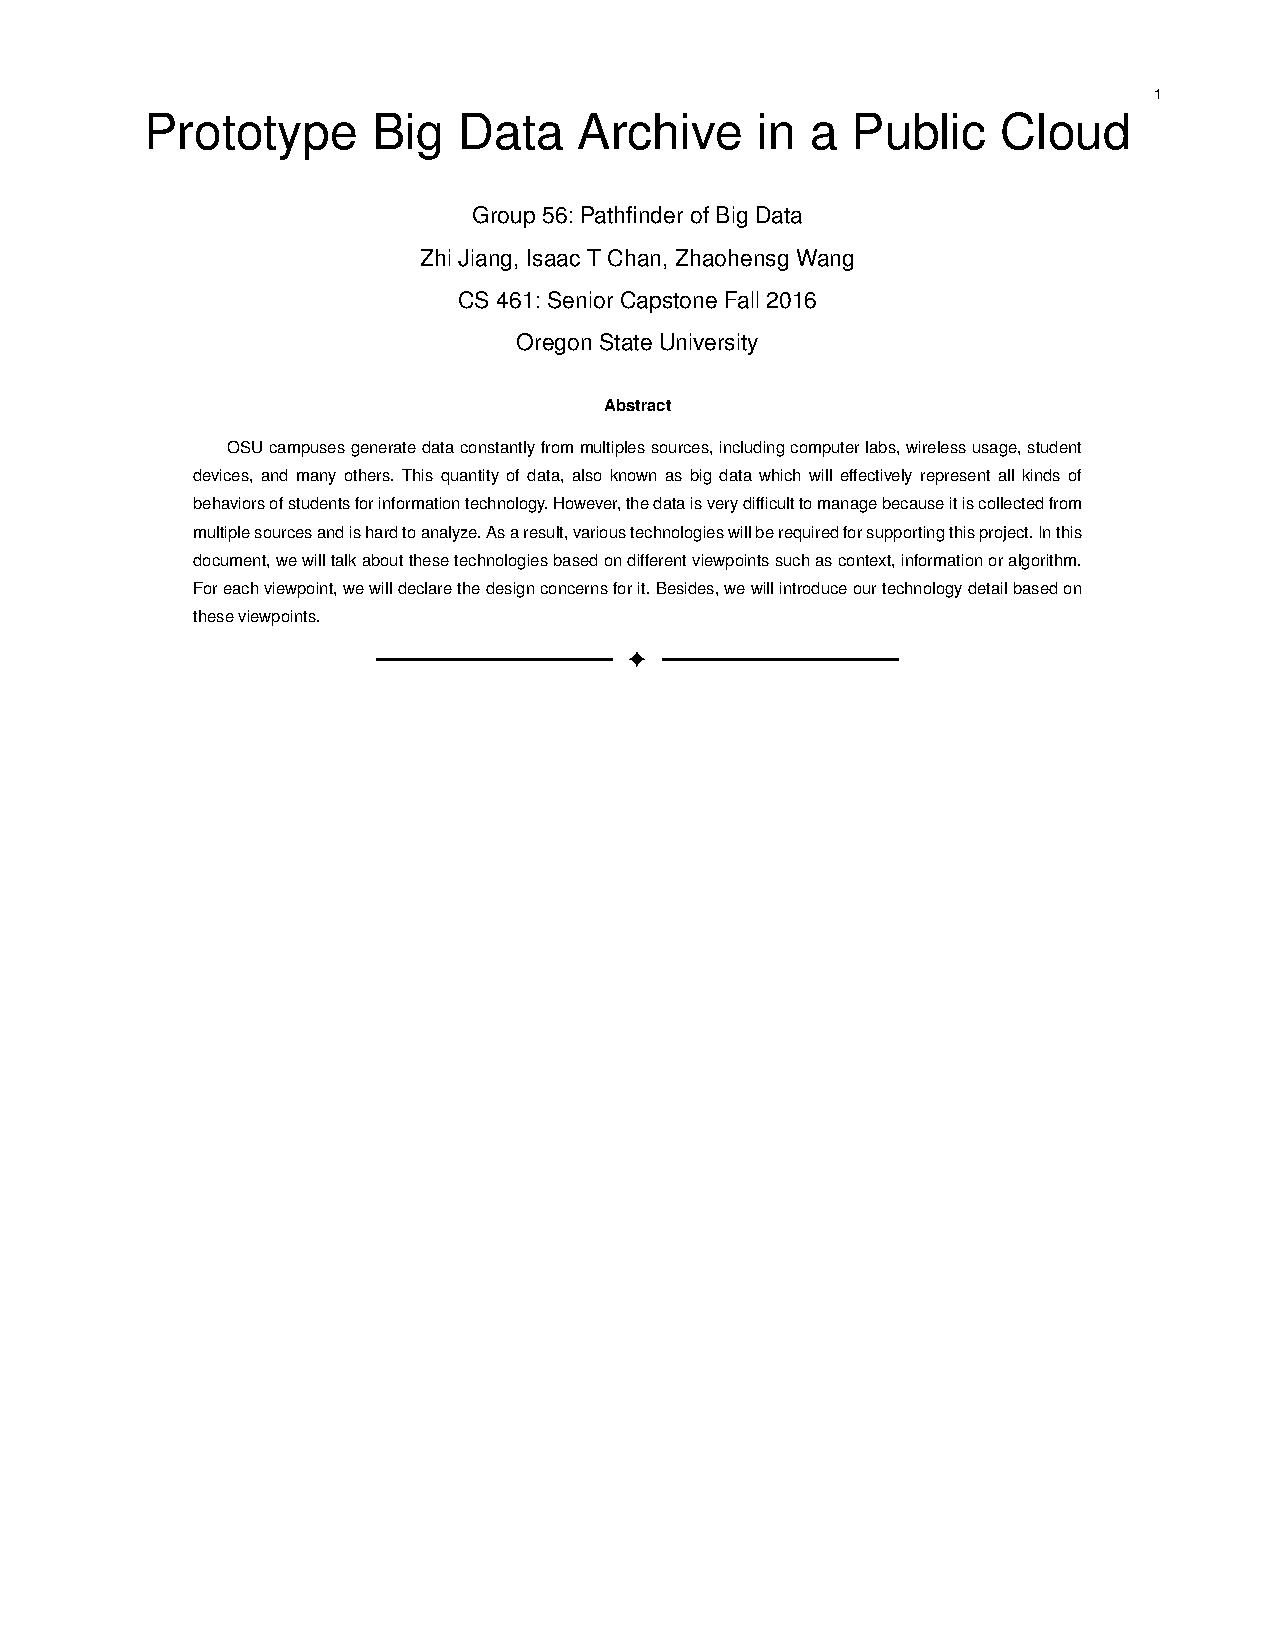
\includepdf[pages=-]{Original_Doc/original_design.pdf}
	\subsection{Design Revision}
We changed Amazon Kinesis to AWS SDK. We found Amazon Kinesis is a useful tool for the data stream, but data our client provided is formatted. On the other hand, for some reasons, we were authorized completely to use AWS EMR, so we were not able to use some services. Python is a good choice for us because we are more familiar with it. The AWS provides a package of Python, and which includes many useful functions to complete our requirements such as downloading files from data storage or creating table into database.\\ 

\noindent On the other hand, we didn’t use Data Pipeline. The reason we chose this tool is we would like to implement automation. The advantage of Data Pipeline is it can make a schedule for some specific tasks, so this point satisfies our needs. Eventually, we gave up this tool because when we used Python, we found it can also implement automation for the entire project.\\

\noindent We discuss the process with our data analyst for loading data and we find that a graph of the workflow will better represent the steps for loading new data. Because of this, we add the workflow for loading the new data from S3 into the DynamoDB.Furthermore, we also make some changes for implementing DynamoDB table. Instead of using Java APIs, we use the boto3 which is the Python SDK to implement the table in DynamoDB.The reason is the boto3 provides specific steps for loading data from S3 into DynamoDB by using EC2 instances.\\

    \newpage
    \setcounter{section}{4}
\section{Weekly Blogs}
	\subsection{Fall Term}
\subsubsection{Week 3}

\textbf{Zhi Jiang}\\
\noindent\textit{Progress since last week:}\\
Last week we completed the first assignment problem statement. The assignment effectively made me understand the entire condition of this project. This assignment helped me quickly collect all kinds of information about this project. On the other hand, I still learned two kinds of markup languages, and which are LaTex and Markdown. These markup languages will be useful tool for I working this project.\\

\noindent\textit{Any problems you encountered:}\\
\noindent The most important problem we encountered is database. According to client's comments, we need to evaluate some ways to implement NoSQL database, but actually we are not familiar with database. I spent a lot of time on searching materials about NoSQL database when I modified our problem statement. Another problem is we should have more effective communication with the client. The Client told us it would be a good idea to let him know of deadlines, so we should ensure information symmetry for client.\\

\noindent\textit{Plans for the coming week:}\\
\noindent We will keep going to focus on database in next week. I will try to send email to my instructor in CS 340 and ask him some questions about NoSQL and way of implementation of NoSQL. We will find more details in this project, in the other words, we will do a complete analysis for it. \\

\noindent\textbf{Isaac T Chan}\\
\noindent\textit{Progress since last week:}\\
\noindent Last week we wrote the problem statement and sent it and received it from the client. There was only one revision necessary which was good, meaning we understand the problem that he presented fairly accurately.\\

\noindent\textit{Any problems you encountered:}\\
\noindent We somehow got a bit behind on deadlines and sent it to the client too late. However he was very good about reading and signing it so we were lucky in that respect. We will be much more prompt in the future.\\

\noindent \textit{Plans for the coming week:}\\
\noindent I don't know the difference between relational and non-relational databases and need to learn. We will probably want to fill in the gaps in our personal knowledge and start thinking about a plan to implement.\\

\noindent\textbf{Zhaoheng Wang}\\
\noindent\textit{The process we finish last week:}\\
\noindent We finish our problem statement part. So I figure out the general process of project about what should we do and how to evaluate whether our project meets the requirements.However,it is not specific enough.\\

\noindent\textit{Any problems you encountered:}\\
Our project requires to use the amazon web service as an platform. However, I never use it before and I am not familiar with this platform. Besides, I am still confused about the concept of NoSQL database.\\

\noindent\textit{Plans for the coming week:}\\
Firstly, I would like to search more information about this platform about how to use the AWS. Secondly, our project will focus on collecting data, organizing and analyzing data and implement the database to store the data. Therefore, I should figure out how to implement a NoSQL database on AWS.Furthermore,I might search some videos about what is the difference between NoSQL and SQL.\\

\subsubsection{Week 4}

\textbf{Zhi Jiang}\\
\noindent\textit{Progress since last week:}\\
In the last week, we have done three things. First one is we fixed some minor mistakes in problem statement according to instructor's feedback. Secondly, we sent our modified document to client and made an appointment with him in next week. Third thing is we met with our TA and talked somethings about requirements documents. As for me, I reviewed some commands of Git because I think I am not familiar to this tool.\\

\noindent\textit{Any problems encountered:}\\
The most important problem we encountered should be we still have a lot of problems about our project, in the other word, we need more details such as implementation of database and types of sample data.\\ 

\noindent\textit{Plans for the coming week:}\\
We will focus on requirements document in next week.  As I mentioned above, we made an appointment with our client in next week because we need more specific information about project. After meeting with client, we will start to do requirements document. We will read related material and understand how to write correctly requirements. For instance, we need to know differences between functional requirements and non-functional requirements.\\

\noindent\textbf{Isaac T Chan}\\
\noindent\textit{Progress since last week:}\\
There was not a lot of progress this last week. Because of the extended revision deadline for the problem statement, we were on hold until we received feedback for it. When we did receive feedback, it required very minimal corrections before we sent it again to our client. We also met with our TA for the first time, made plans for meeting with our client, and have a plan for the requirements document, due next week.\\

\noindent\textit{Any problems encountered:}\\
There were no problems we encountered. I did worry a little about the condition of our problem statement because we had only a short time to fix problems and get it approved and signed by our client, but was relieved to see that the feedback was positive.\\

\noindent\textit{Plans for the coming week:}\\
This next week will be busy. The requirements document seems to need a lot of work. I am not that experienced in LaTeX - some time will be spent on the IEEE formatting. Additionally, we hope to meet with our client as early in the week as possible, so we can clarify some details and be ready to write an excellent requirements document.\\ 

\noindent\textbf{Zhaoheng Wang}\\
\noindent\textit{Progress since last week:}\\
In the last week, we revise our problem statement base on the feedback. After that, we send it to our client to check whether fits the requirement about the project. Besides, we meet our TA on Friday. we go though the general process about future meeting and we also ask several question about requirement document such as how detail should our requirement document should be. Furthermore, I do some research about NOSQL database which required by our project. it seems the biggest difference between SQL and NOSQL is SQL database uses the table and the NOSQL uses the document. The NOSQL is more focus on availability and performance.\\     

\noindent\textit{Any problems encountered:}\\
For the requirements document, the lecture shows five general parts about what we need to write such as functionality, security, response time. However, i could not give a clear answer for several parts such as security. For example, we are going to use the database on AWS. Usually, there will be some disaster recovery for the database and we might figure out how to do it.\\   

\noindent\textit{Plans for the coming week:}\\
we are going to have a meeting with our client and figure out how to organize our requirements document. Additionally,I am not familiar with latex style so i would like do some research on it. Furthermore, if I have enough time after finishing the requirements document and the research about latex, I will focus on searching the information about how to use Amazon Web Services.

\subsubsection{Week 5}

\textbf{Zhi Jiang}\\
\noindent\textit{Progress since last week:}\\
In this week, we finished the final draft of problem statement and started to write software requirement specification. This document needs more details about requirements, thus we met our TA again and then we gained many information. In process of writing document, we feel benefits of requirement specification, because we need to completely understand what we do in project, and provide some specific plans to each part, otherwise we cannot complete this document very well.\\ 

\noindent\textit{Any problems encountered:}\\
The third part of document "the specific requirements" is main problem we encountered, because we still have many questions about this part such as interfaces and functional requirements. In fact, according to client's introduction, our project is not very complex and the main part is database, so we will consider which section need to be ignored in this document.\\

\noindent\textit{Plans for the coming week:}\\
The document is due next week, so the primary task for us is complete this document bases on feedback of TA and client. Probably we need to search more material about database, and find useful information for specific requirements.\\

\noindent\textbf{Isaac T Chan}\\
\noindent\textit{Progress since last week:}\\
This week we completed our rough draft of the requirements document. We realized early that there were some requirement details that we didn't know; we met with our client early on to define them. Then we wrote the rough draft and gave it to our client to check the content.\\

\noindent\textit{Any problems encountered:}\\
We still need to put the document into IEEE format. Also, there was some confusion regarding the "specific requirements" section of the document. It seems like we've covered all the requirements already in the previous section. This is likely an organizational issue and we will need to figure it out.\\

\noindent\textit{Plans for the coming week:}\\
Luckily we have another week to turn in the final draft. We will need to put it into IEEE format. Regarding the missing section, we may need to meet with an instructor or TA to reorganize our document. Finally we need to finish it before Friday so we will have enough time to verify requirements one last time with our client, get it signed, and turn it in.\\

\noindent\textbf{Zhaoheng Wang}\\
\noindent\textit{Progress since last week:}\\
This week we have finished our rough draft of requirements document and we send it to the client in order to get some feedback. After that, we revised it base on the feedback form client.Then,we send it to our TA in order to get more feedback.Besides, I have do some research about the idea between cloud platform ,PaaS and IaaS.The cloud platform is using the cloud computing technology. The Platform as a service (PaaS) offered by cloud platform will provide ​a development environment for the product including OS, compiling and execution environment of programming language.The Infrastructure as a service(​IaaS)​ will ​abstract the details of infrastructure​ such as ​physical computing resources​, security.Thus, the user don’t need to worry about managing ​cloud infrastructure\\    

\noindent\textit{Any problems encountered:}\\
we have some question about the specific requirement part in requirements document. Because, we are not clearly figure out all the specific functions we need to use yet.\\

\noindent\textit{Plans for the coming week:}\\
Next week, we will do some revision after getting the feedback from TA. Then, send it to our client to check whether fit his requirement. Besides, I would like to do some research about some analyze tool such as tableau because our project need to have some basic reporting and analyzing functionality.    

\subsubsection{Week 6}

\textbf{Zhi Jiang}\\
\noindent\textit{Progress since last week:}\\
In this week, we talked grade of problem statement with Kirsten, and she gave us some useful suggestions about writing structure. We will do appropriate adjustment for our problem statement through her comments. Secondly, we finished the requirements document but our TA thinks it is not good enough. He thinks we need more stuffs in "Specific requirements" section. I still learned some knowledge about technology when I was doing the requirements document. I download the document of Dynamo DB for developer and read it. I find that it has provided some APIs of basic operations of NoSQL Database. These APIs will make our tasks more convenient.\\

\noindent\textit{Any problems encountered:}\\
 The problem we need to solve are mistakes in the requirements document. We have to change our format of Latex and we also need to provide more details for functional requirements according to TA feedback. So it means we need to do more research about NoSQL database and completely understand its functions.\\

\noindent\textit{Plans for the coming week:}\\
We will modify our requirements document as soon as possible and return it to client and TA. We still need to learn more thing about NoSQL.\\

\noindent\textbf{Isaac T Chan}\\
\noindent\textit{Progress since last week:}\\
This week we received our graded problem statement back and finished up the final draft of our requirements document. We made an appointment with Kirsten to talk about our problem statement grade and the "specific requirements" section of our requirements document. We plan to reorganize and resubmit our problem statement, because the content was good but the structure was poorly designed.\\

\noindent\textit{Any problems encountered:}\\
Our requirements document is likely not in "final draft" shape. We received feedback from our client, who thinks it is good, and also our TA, who thinks it is not so good. Due to the delay of feedback we may need to get an extension and turn it in at a later date.\\

\noindent\textit{Plans for the coming week:}\\
 Probably will need to finish up the requirements document and restructure the problem statement. Plus any new assignments.\\

\noindent\textbf{Zhaoheng Wang}\\
\noindent\textit{Progress since last week:}\\
In this week, we make an appointment with Kirsten about our problem statement and get useful feedback from her. we find that our problem statement need to organize the information more clearly for the readers. Besides, we finish our requirements document and get some feedback from our TA. Furthermore, i do some research about the whole process again and i have a more clearly idea about how this whole process goes.\\

\noindent\textit{Any problems encountered:}\\
Our requirements document still have some problems: 1. The syntax for latex need to change 2. The content for specific requirements part should be more specific 3. The format for specific requirement part need to change 4. Adding a schedule for the requirements\\

\noindent\textit{Plans for the coming week:}\\
We need to revise our Requirements document and problem statement again. Besides, I would like do more research about loading data from different source and the algorithm for searching specific data in a file. i believe this will help a lot for the detail design part.\\

\subsubsection{Week 7}

\textbf{Zhi Jiang}\\
\noindent\textit{Progress since last week:}\\
In this week, the first thing is that we completed the final draft of requirements document. In this process, we add two more sections "Hardware interface" and "Software interface". We added more details for functional requirements. Eventually we created our schedule bases on functional requirements. On the other hand, I started to prepare for writing technology review. I have found many materials about each piece I will deal with so they will be useful for me to complete this assignment.\\

\noindent\textit{Any problems encountered:}\\
Actually, when I read those materials about my pieces, I was frustrated, because there are many concepts I don't know. It is hard to understand relationship between some technologies, so I believe that this is the biggest problem I encountered.\\

\noindent\textit{Plans for the coming week:}\\
In next week, we will start to do technology review, so it means we must understand completely all pieces in our product, so probably we need to find more materials or ask corresponding questions to TA or instructor.\\

\noindent\textbf{Isaac T Chan}\\
\noindent\textit{Progress since last week:}\\
We completed the final draft of our requirements document. We added functional requirements, software system attributes, and added more details for performance metrics. We also added a rough schedule based on our functional requirements. There is a rough outline of our technology review.\\

\noindent\textit{Any problems encountered:}\\
In researching for the technology review, I found that with the information we have right now about the data and the system, it is difficult to envision the final product. I think we need to get a sample of data to work with, or all of our design and reviews are just speculation and our final product could deviate far from the preliminary design.\\

\noindent\textit{Plans for the coming week:}\\
We plan to finish our technology review and start the design document. We will need more details on the design document and may need intermediate meetings with our TA to make sure we're doing it correctly.\\

\noindent\textbf{Zhaoheng Wang}\\
\noindent\textit{Progress since last week:}\\
In this week, we revise our Requirements document again base on our TA's feedback. We first change the functional requirement part and make this part more detail. Besides, we add performance requirement part and system attribute part which let reader understand our system more clearly. Furthermore, we make a schedule in gantt chart which give a clearly schedule for our project.\\

\noindent\textit{Any problems encountered:}\\
For the technology review, i am not familiar with how to make the data suitable before visualization so i need to do more research about this part. Besides, i also need to figure out what kind of tools we might use for visualization.\\

\noindent\textit{Plans for the coming week:}\\
we might start our detail design next week. Therefore, it is better to ask an appointment with our client and data analyzer. we need to check our thought with our client and make sure it fits our client's requirement. For example, we need to ask for some sample data from our client so we could figure out the detail process for loading data. Besides, we also need to check our thought with our user(data analyzer) and figure out what types of data we need to create for loading into the analyze tool.\\

\subsubsection{Week 8}

\textbf{Zhi Jiang}\\
\noindent\textit{Progress since last week:}\\
We completed technology review and submitted it on Monday. And then we started to do the design document. In this document, we need to focus on how to implement technologies we discussed in the last document. When we met our TA today, we asked some question about our technologies such as what's the difference between data storage and database. TA given us useful suggestions and explanation. And he also provided some basic ideas of big data,so these are good reminders for us to consider the whole product.\\

\noindent\textit{Any problems encountered:}\\
The problem is also how we implement these technologies. We need to do more research base on suggestions of TA because we are not familiar with some technologies like the filesystem.\\

\noindent\textit{Plans for the coming week:}\\
 As for next week, probably we will meet with our client and talk something about sample data. According to TA's suggestion, we should get sample data as soon as possible because we need to design our product depends on characteristics of these data. On the other hand, we will make a video for our product.\\

\noindent\textbf{Isaac T Chan}\\
\noindent\textit{Progress since last week:}\\
This week we finished our technology review. Not a lot was discovered because we had previously researched technologies we would use, and our research affirmed those technologies. Additionally, I think we found that, because our client requires us to use AWS, AWS actually offers a lot of the technologies we need. This is very helpful because it reduces the complexity of our implementation.\\

\noindent\textit{Any problems encountered:}\\
Our problems remain the same as last week. We still need a sample of the data to determine specific implementation details and how to design the database.\\

\noindent\textit{Plans for the coming week:}\\
I plan on restructuring our problem statement next week and resubmitting it. I also plan on completing a portion of the design document. I think that we have fallen behind schedule slightly and I think the progress report presentation will take more time than we think. As it's already the end of week 8, we have a lot of work ahead.\\

\noindent\textbf{Zhaoheng Wang}\\
\noindent\textit{Progress since last week:}\\
 on this week, i finish our technology plan which is going to figure out the optimal options for achieving the requirements. This document is a necessary step for our design documents and it is very important. In this document, i choose three pieces of technologies: the first one is to figure out which is the optimal option of the storage way for dealing with processed data. In this part, i compare the other storage way with database. After that,I compare the sql and nosql database. Finally, I compare three types of nosql databases.because of the research, I benefit a lot and get more clearly understanding for the features of database than before.\\
 
\noindent\textit{Any problems encountered:}\\
 i am going to start our design document however there are several things we have to check with our client: 1 i need to get some sample data first because our first step is to parse the file. 2 i need to figure out the information we need to store. 3 For the visualization part, i need to check with data analyzer because he is our user.\\
 
\noindent\textit{Plans for the coming week:}\\
we are planning to have an appointment with our client next week and figure out the questions above.Besides, there are many research for our project. it is very important to get a clear scope of our project before we start to design it. furthermore, we should start to think about the progress report on next week.
\\\textbf{}

\subsubsection{Week 9}

\textbf{Zhi Jiang}\\
\noindent\textit{Progress since last week:}\\
In this week, we met with our client on Monday. The main thing we talked is about sample data. We are doing the design plan for entire product, so sample data can let us understand how to design each part. Another important thing was we completed the revision of problem statement and submitted to Winters. As for myself, we found more information about solution I chose for my parts. I read some developer guide provided by AWS and known some basic idea for building Hadoop framework.\\

\noindent\textit{Any problems encountered:}\\
The problem we encountered is we have not got sample data from our client, so it will affect our plan, because sample data is very important for us and all of tasks we will do must depend on sample data.\\

\noindent\textit{Plans for the coming week:}\\
The primary is to get sample data for comping week and then complete design plan as soon as possible. I got grade for my technology review, and I will probably talk feedback with Winters in next week.\\

\noindent\textbf{Isaac T Chan}\\
\noindent\textit{Progress since last week:}\\
We met with our client early in the week and requested a set of sample data. This is very important for the design document because our database structure depends on how the sample data is set up. There are many components that are reliant on the sample data, such as whether or not we need to cleanse, parse, or otherwise process the data before it can be stored in the database. We also restructured our problem statement and sent it to Dr. Winters.\\

\noindent\textit{Any problems encountered:}\\
We are waiting for the set of sample data from our client. Due to the break, we don't know when to expect it but as soon as it does we can inspect it and base some design decisions off of it.\\

\noindent\textit{Plans for the coming week:}\\
Hopefully we receive the set of data as soon as possible. Then we can organize and collaborate on the design document. Additionally at some point we should write the progress report and begin the presentation.\\

\noindent\textbf{Zhaoheng Wang}\\
\noindent\textit{Progress since last week:}\\
This week we make an appointment with our client and ask for a sample data. The sample data is very important for design document because if we get the sample data then we will figure out the data type we should parse for our project. Besides, the sample data will give a good example about the information we should store into database. I also watch some video about how dynamodb works however it is not very helpful.\\

\noindent\textit{Any problems encountered:}\\
The problem is i still confuse about the way that dynamodb store and there are several questions i need to figure out: 1. Does dynamodb requires er diagram? 2. How quicksight works on aws? 3. How to achieve the functionality for database? another thing is we don't get our sample and we could not start our design part.\\

\noindent\textit{Plans for the coming week:}\\
Once we get the sample data, it is time to start our design document. Furthermore, we might also start to think about the process report and think about how to organize it.

\subsubsection{Week 10}
\textbf{Zhi Jiang}\\
\noindent\textit{Progress since last week:}\\
In this week, we gained the sample data from our client and then completed the design document. According to this document, we understand more details about our technologies. We also made a new timeline in this document because there are some changes which are different from previous documents.\\

\noindent\textit{Any problems encountered:}\\
The most difficult problem is also about our technologies. We still need to spend more time to learn how to use these technologies. I think we can start to use sample data to attempt some basic functions for tools on AWS.\\

\noindent\textit{Plans for the coming week:}\\
We plan to complete the last assignment on Sunday. And we still need to submit the hard copy with signature as soon as possible.\\ 

\noindent\textbf{Isaac T Chan}\\
\noindent\textit{Progress since last week:}\\
This week we completed our design document. In the beginning of the week we received a sample of data from our client. This data was in a CSV format, which should be simple to load into the database. During our work with the design document, we learned much more about the technologies we will implement. After seeing the format of the data and what types of fields it contains, it made me more confident in my technology choices because I had no conflicts with the data.\\

\noindent\textit{Any problems encountered:}\\
I think that we are still in hypothetical terms when designing our project. The problems we will encounter will be small nuances in the technologies we choose. As of now, I don't think any of us have issues with our technologies or the sample data, but the issues we may have are very difficult to identify without actually implementing the project. Now that we have sample data, we can probably begin to work with it on AWS and experiment, but we will need credentials given to us by our client.\\

\noindent\textit{Plans for the coming week:}\\
We plan to complete the progress report on Sunday, 12/4. Also we submitted an unsigned version of the design document and will need to submit the signed version as soon as it is returned to us.\\

\noindent\textbf{Zhaoheng Wang}\\
\noindent\textit{Progress since last week:}\\
This week, we receive our sample data and finish our preliminary design document.In this document, we introduce our technology based on various such as context viewpoint,algorithm viewpoint and information viewpoint.This document gives us more clear visual for our project.Besides,I have done some personal research about the process for designing NoSQL table.Usually, the relational database table will design by ER-diagram but the ER-diagram is not suitable for represent NoSQL database table.However, the ER-diagram can convert to the NoSQL database table model.Therefore, we can create the ER-diagram first and convert it into the NoSQL database table model.\\

\noindent\textit{Any problems encountered:}\\
The sample data provided by data analyzer is in csv file type which is already readable by using excel.In this file, it contains the data such as userid,time,terminal type, OS and others.Therefore, there will be two things I need to check with data analyzer.The first thing is whether the future data is the same type with the sample data. The second thing is whether the sample data contains all the information we need to store.\\

\noindent\textit{Plans for the coming week:}\\
In the next week, we will finish our process document for this term. Besides, I might start to think the specific step about how to implement this project.\\
    \subsection{Winter Term}
\subsubsection{Week 2}
\textbf{Zhi Jiang}\\
\noindent\textit{Progress since last week:}\\
In this last week, we met with our TA on Wednesday and we talked something about our project. Actually, we have not yet got the account for Amazon Web Services, because our client explained that they cannot access to the cost and billing alters so they have to solve this problem before we gain account. As for myself, I read all documents we completed in this week because I want to review more details about our project.\\

\noindent\textit{Any problems encountered:}\\
Obviously, the problem we encountered is the AWS account, we hope we can get it as soon as possible.\\

\noindent\textit{Plans for the coming week:}\\
We are planning to connect our client with the account. On the other hand, we should start to work on our project bases on the schedule we made before.\\

\noindent\textbf{Isaac T Chan}\\
\noindent\textit{Progress since last week:}\\
The week before last, we contacted our client for details regarding our AWS account access. We received a reply last week, explaining the difficulties our client is having with billing. We sent another email explaining the urgency and how we are behind schedule.\\

\noindent\textit{Any problems encountered:}\\
We are now 2 weeks behind schedule and need to accelerate as soon as we get access to AWS and the data.\\

\noindent\textit{Plans for the coming week:}\\
Hopefully we receive AWS account access and will begin development as soon as we do.\\

\noindent\textbf{Zhaoheng Wang}\\
\noindent\textit{Progress since last week:}\\
In this week, we schedule our group meeting with our TA and we talk about our current process of our project. Unfortunately, we don't get the AWS account access and the data from our client.As a result, some important step can not start yet. we have send an email with our client to check about this problem.\\

\noindent\textit{Any problems encountered:}\\
we are waiting for client's email and personally i would like to do some research about this project.\\

\noindent\textit{Plans for the coming week:}\\
we don't get the account for AWS which is necessary for our project. Besides, i am still unsure for some of the detail for the project.\\

\subsubsection{Week 3}
\textbf{Zhi Jiang}\\
\noindent\textit{Progress since last week:}\\
The good news for us is we get the access to AWS in this week, so which means we can start to work on our project formally. My task is to transform data from data storage to database in this project, so I read some developer guides for tools I probably use.\\

\noindent\textit{Any problems encountered:}\\
I think the problem is I am not familiar with these tools. In my task, I will use a tool call “EMR”, and it is a little bit complex, so I think I should spend more time to understand it.\\

\noindent\textit{Plans for the coming week:}\\
I will start to work on my task in this weekend, and I will continue reading material for them. If I have any questions I will send email to TA or technical adviser of our client. Finally, I hope I can gain some progress before the next weekend.\\

\noindent\textbf{Isaac T Chan}\\
\noindent\textit{Progress since last week:}\\
We got access to AWS this week and have emailed our client for access to the specific tools we require. I reviewed the documents for a refresher for the tasks I'm assigned.\\

\noindent\textit{Any problems encountered:}\\
I don't have any issues aside from delayed access to AWS. However, I find that most of my assigned tasks are after the majority of the work (alpha release will work without my contributions) so I want to work with my group on their tasks so I can keep up with the progress.\\

\noindent\textit{Plans for the coming week:}\\
I want to try loading sample data into the database. It seems that our knowledge about NoSQL tables is lacking and I think that trying to load the data in will help my overall understanding.\\

\noindent\textbf{Zhaoheng Wang}\\
\noindent\textit{Progress since last week:}\\
In this week, we schedule an appointment with our client on Tuesday. After that, we get the access account for our project.On Wednesday, we meet our TA and we talk about the current progress for our project. On Thursday,we send the email for asking the permission for the software such as S3, Dynamodb and quicksight.\\

\noindent\textit{Any problems encountered:}\\
Now, we don't have the problem yet seems we just have the permission for access the software.\\

\noindent\textit{Plans for the coming week:}\\
For next week, we would like to start our project as soon as possible. It seems our progress is behind the schedule.\\

\subsubsection{Week 4}
\textbf{Zhi Jiang}\\
\noindent\textit{Progress since last week:}\\
In this week, the first thing is we have gained tools we need from our client. We started to discuss a specific plan for next step. And we will start to modify our design document because actually some tools and solutions are different from what we planned before.\\

\noindent\textit{Any problems encountered:}\\
The problem for me is I cannot create a cluster successfully because we lack a tool called IAM. I have reported this issue to our client on Friday. I hope it can be solved as soon as possible, otherwise, we could not do next step.\\

\noindent\textit{Plans for the coming week:}\\
We will show some results for our TA in next week, Which is we will import data from S3 to Dynamo. This is the very important step in the whole project because all of the unprocessed files will be stored in S3.\\

\noindent\textbf{Isaac T Chan}\\
\noindent\textit{Progress since last week:}\\
This week we have obtained access to almost every AWS utility we will need. We tested some of them out and realized that our understanding of the utilities was flawed as we were writing the preliminary design documents. We have come up with a plan to tackle the rest of the project.\\

\noindent\textit{Any problems encountered:}\\
No problems really, in fact this week we realized we aren't as far behind in the schedule as we thought so things are going well.\\

\noindent\textit{Plans for the coming week:}\\
Our group plans to have a working meeting next week. We will load some data into DynamoDB using a python script executed on an EMR or EC2 cluster, then demonstrate this to our TA. Additionally, I'm keeping note of the changes that I'll need to make to our design document before the end of the term.\\

\noindent\textbf{Zhaoheng Wang}\\
\noindent\textit{Progress since last week:}\\
On this week, we have the group discussion on Wednesday and we discuss our project current process and the next step for our project. after that, we meet with our TA to talk about our project and the future plan. This week, we all access the AWS server in order to get familiar with our project and after trying some software, we find we might make some changes for our project.\\

\noindent\textit{Any problems encountered:}\\
We need to do some preparation for loading data and we are catching up our schedule.\\

\noindent\textit{Plans for the coming week:}\\
For the following week, our group plan to load the data from S3 into the DynamoDB by using EMR. We plan to load some sample data into the DynamoDB. If the sample data works, the data we load in the future should be working. After that, we will show it with TA to get some feedback.\\

\subsubsection{Week 5}
\textbf{Zhi Jiang}\\
\noindent\textit{Progress since last week:}\\
In this week, TA canceled the meeting, so we did not meet with her on Monday. Another thing is that I completed the wired assignment. I still introduced our project to my partner.\\

\noindent\textit{Any problems encountered:}\\
There is no any problem so far.\\

\noindent\textit{Plans for the coming week:}\\
I will finish midterm progress report in next week.\\

\noindent\textbf{Isaac T Chan}\\
\noindent\textit{Progress since last week:}\\
This week we submitted our poster for printing after we got it client/instructor approved. I continued to work with the data analyst to connect to EMR and gained access. After gaining access, I ran the code provided, after making modifications for it to work within the AWS environment. None of this needed to be documented, as it was a proof of feasibility for our client's benefit and to ensure our project is finished.\\

\noindent\textit{Any problems encountered:}\\
Haven't received usage estimates.\\

\noindent\textit{Plans for the coming week:}\\
I still haven't received an estimate for future usage so I can't complete the cost comparison. I'll plan on sending a follow-up email for those numbers if I don't receive them by Monday. I think next week the midterm progress report is due, so I'll do that next week.\\

\noindent\textbf{Zhaoheng Wang}\\
\noindent\textit{Progress since last week:}\\
On this week, I introduce the project of my group with the classmate that instructor assigns for the WRIED card assignment. We have a short discussion with our projects. The project of him is about the mobile app which is designing for guiding the tourists. The users could easily access to map without internet connection on this app. It is very useful and it is cheap for the users. Besides, he also introduces the feature of this app. For example, there will be a website which is designing for uploading videos and feedback for the viewpoints. Another thing I do this week is to update the images for workflow and make it clearly.\\

\noindent\textit{Any problems encountered:}\\
Currently, There is no any problem for me.\\

\noindent\textit{Plans for the coming week:}\\
For the next week, the midterm report will come soon. So I plan to start to writing the midterm report. Besides, I would like to introduce my project again with the partner who assigned for WRIED card assignment. Because I think some of the point I introduce is not very clear.

\subsubsection{Week 6}
\textbf{Zhi Jiang}\\
\noindent\textit{Progress since last week:}\\
In this week, we have completed the midterm progress presentation and report. In presentation, we showed off our project at some alpha level functionalities such as importing data and visualization of data. On the other hand, we have revised some documents includes Requirement Document and Technology Review. Finally, we created OneNote and organized all materials and documents on OneNote.\\

\noindent\textit{Any problems encountered:}\\
In this week, I did not encounter any problems.\\

\noindent\textit{Plans for the coming week:}\\
In this week, we have completed the midterm progress presentation and report. In presentation, we showed off our project at some alpha level functionalities such as importing data and visualization of data. On the other hand, we have revised some documents includes Requirement Document and Technology Review. Finally, we created OneNote and organized all materials and documents on OneNote.\\

\noindent\textbf{Isaac T Chan}\\
\noindent\textit{Progress since last week:}\\
This week, we scrambled to complete all the requirements for the midterm progress report. This included meeting to record our presentation, revising documents, and completing the OneNote. In the OneNote, we added an organizational scheme for our poster.\\

\noindent\textit{Any problems encountered:}\\
Not really. Probably just need to talk to our client and data analyzer to be ready to implement my portions.\\

\noindent\textit{Plans for the coming week:}\\
During my review of my midterm progress, I realized that I hadn't done much personally regarding the project due to our task division. Actually there are still a few more weeks before I'm scheduled to begin my portions (have to begin after we have a working solution). But there's many requirements I need to work on my tasks, including getting data from our client and consulting with the data analyzer to see what kinds of analysis we should try.\\

\noindent\textbf{Zhaoheng Wang}\\
\noindent\textit{Progress since last week:}\\
This week,we first revise our review document and the design document. After that,we finish our presentation slide on Monday night and we schedule a group appointment with each other on Tuesday in order to finish our presentation. Our video is around 20 mins. it is a little short in our project. As a result, we check it with TA on Wednesday.After that, we start our progress report on Wednesday night. After finishing the progress report, we need to make a simple structure of the poster.\\

\noindent\textit{Any problems encountered:}\\
1. Check with data analysis whether there is an efficient way for organizing table 2. Figure out which sample data can be ignored

\noindent\textit{Plans for the coming week:}\\
There still have some improvement for these parts in our project. Firstly, the way I choose for design the data structure may not be the optimal choice. Therefore, I would like to check with the data analyzer whether it is the efficient way or not. Secondly, the graph which made by QuickSight needs to improve because some of sample data needs to be filter. Furthermore, the QuickSight seems not handle the complex analysis and our client doesn’t give specific topic that we need to analysis. As a result, I would like to check with the data analyzer what kind of analysis we need to do\\

\subsubsection{Week 7}
\textbf{Zhi Jiang}\\
\noindent\textit{Progress since last week:}\\
In this week, I started to improve my portion. On the other hand, we send design document to our client for signature, because we did some changes on it.\\

\noindent\textit{Any problems encountered:}\\
We did not get the signature on time, so I just hope we can get it as soon as possible.\\

\noindent\textit{Plans for the coming week:}\\
In the next week, I think we should have an appointment with our client because we should report to our client what we did in several weeks ago specifically. I will continue to improve my portion and test it.\\

\noindent\textbf{Isaac T Chan}\\
\noindent\textit{Progress since last week:}\\
This week we sent our updated design document to our client for approval and signature.\\

\noindent\textit{Any problems encountered:}\\
We haven't yet received a signature for the design document from our client and need to submit it by today.\\

\noindent\textit{Plans for the coming week:}\\
This coming week I need to contact our client and data analyzer for approval on the strategies I want to employ for data analysis and performance testing. This involves getting larger sets of sample data than we have received so far so there might be some issues regarding how much data they are willing to give us.\\

\noindent\textbf{Zhaoheng Wang}\\
\noindent\textit{Progress since last week:}\\
On this week, we meet with our TA on Wednesday to talk about the current process of our project and we send our design document to our client for asking the signature.\\

\noindent\textit{Any problems encountered:}\\
we don't get the signature for the new design document and we will send an email to TA. Hopefully, we could get the signature as soon as possible.\\

\noindent\textit{Plans for the coming week:}\\
For next week, we are planing to have an appointment with our client in order to check whether we are on the correct position. Besides, we might optimize our project. For example, the table can be optimized by creating three separate tables. By doing this way, some important data can be store more security.\\

\subsubsection{Week 8}
\textbf{Zhi Jiang}\\
\noindent\textit{Progress since last week:}\\
First of all, I continued to improve my portion, but I did not complete it. Secondly, we got the signature from the client for the design document. On the other hand, we met with our data analyzer, and she gave us some suggestions about this project. On important thing is we should create three tables when we import data from S3 to dynamoDB.\\

\noindent\textit{Any problems encountered:}\\
The problem I encountered is I did not complete function to create a table automatically. In this library, it has fixed format to create a table, so I was not able to use loop statement for setting name of each attribute.\\

\noindent\textit{Plans for the coming week:}\\
In next week, we will try our best to implement the solution based on data analyzer's suggestion. On the other hand, we still have a class meeting with our instructor, so probably we should discuss how to show our project in class.\\

\noindent\textbf{Isaac T Chan}\\
\noindent\textit{Progress since last week:}\\
This week we received our signed design document from our client. He included a suggestion to meet with the data analyzer, which we were already planning to do. After meeting with her on Wednesday, we got several suggestions about the pipeline from S3 to the database, and creating two other tables with identifiable data (MAC address, ONID) with a hashed unique key to tie them back to the main data. This is something we will implement with fake ONID and MAC address, due to the sensitivity of the data.\\

\noindent\textit{Any problems encountered:}\\
No problems this week.\\

\noindent\textit{Plans for the coming week:}\\
The data analyzer gave us some suggestions that we plan to implement, including hashed user identifiers and also replicating data to check database performance. She will send us some code to test data analysis as well. Finally we have a class this week on Thursday, so our group should meet and prepare a little bit before presenting in that class.\\

\noindent\textbf{Zhaoheng Wang}\\
\noindent\textit{Progress since last week:}\\
On the Tuesday night of this week, we get signature and the feedback about our design document from our client. On Wednesday, we have an appointment with our TA to discuss our current process. On Thursday, we schedule an appointment with the data analyzer and she gives several suggestion for our project. For example, we would have three table and two of them will be link table which contains Onid,MAC. She also mentions that we would use pipeline to export the data from database.\\

\noindent\textit{Any problems encountered:}\\
Currently, we don't have the problem on this week.\\

\noindent\textit{Plans for the coming week:}\\
On the next week, since the group number of us is 56 we will have the on class group meeting on Thursday.

\subsubsection{Week 9}
\textbf{Zhi Jiang}\\
\noindent\textit{Progress since last week:}\\
In this week, we learned some experiences about Expo in class on Thursday.\\

\noindent\textit{Any problems encountered:}\\
No problems in this week.\\

\noindent\textit{Plans for the coming week:}\\
As for next week, we have a lot of things. We will go to test your program by real data. On the other hand, we need to complete the progress video and progress report, and finally, we have to finish the poster.\\

\noindent\textbf{Isaac T Chan}\\
\noindent\textit{Progress since last week:}\\
This week we met with the TA on Wednesday and discussed the deliverables for the coming week. Then we had class on Thursday and learned more about how to conduct ourselves during expo.\\

\noindent\textit{Any problems encountered:}\\
Aside from requiring real data, nothing. Unless stressing about the million things due in this class counts as a problem.\\

\noindent\textit{Plans for the coming week:}\\
During our meeting with our TA we talked about the current state of the project and I realized that for us to use real data in the expo, even with hashing, we have to have at least one group member able to access to real data. I'll probably send an email to our client/data analyzer and see if we have to meet in person. We also have a meeting on Wednesday of next week to record the final report presentation.\\

\noindent\textbf{Zhaoheng Wang}\\
\noindent\textit{Progress since last week:}\\
On the Tuesday night of this week, we change the table organization base on the suggestion from data analyzer after that we reload the sample data again. On Wednesday, we have an appointment with our TA to discuss our current process and the meeting on Thursday morning. On Thursday, we discuss our project with other group in class time.\\

\noindent\textit{Any problems encountered:}\\
Currently, i have some question about the progress report which is due on the final week.\\

\noindent\textit{Plans for the coming week:}\\
on the next week, we schedule an appointment with group members on Wednesday 3pm to record the video for our project. After that, we are going to discuss the poster for our project since the poster is due on the Friday of week 10.

\subsubsection{Week 10}
\textbf{Zhi Jiang}\\
\noindent\textit{Progress since last week:}\\
We met with our client in this week. We discussed his questions about midterm progress report, also he given us some suggestions for this project. We got a new workflow diagram; this is very important for us because we can improve functions of our project according to this diagram. On the other hand, we still completed the presentation for winter term progress.\\

\noindent\textit{Any problems encountered:}\\
No problems in this week.\\

\noindent\textit{Plans for the coming week:}\\
As for the coming week, we would like complete winter term progress report as soon as possible.\\

\noindent\textbf{Isaac T Chan}\\
\noindent\textit{Progress since last week:}\\
This week, our group met to complete the recording of our presentation. Additionally, we had a meeting with our client to update him on our progress and get a signature for our week 6 progress report. We received a workflow diagram, which was their expectations for our progress. It aligned quite well with our solution, and we plan to update our design document with this workflow.\\

\noindent\textit{Any problems encountered:}\\
There was some miscommunication between our client and us. He had thought that our midterm progress report was the final report, so some of the content didn't make sense with that assumption. We clarified this in our meeting.\\

\noindent\textit{Plans for the coming week:}\\
The next week I plan to complete my individual progress report.\\

\noindent\textbf{Zhaoheng Wang}\\
\noindent\textit{Progress since last week:}\\
On monday, we send the midterm progress report to our client. On Wednesday, we schedule a group meeting from 3pm to 5pm in order to record the video for our project. On Thursday, I schedule an appointment with our instructor to discuss about the final report. After that, i start to write the final report and the poster on Thursday. The poster is due on Friday this week.\\

\noindent\textit{Any problems encountered:}\\
Currently,we don't get the signature for our project. Hopefully, we could get it as soon as possible.\\

\noindent\textit{Plans for the coming week:}\\
For the coming week, i would like to revise my design document again because we get the suggestion from the data analyzer.
    \subsection{Spring Term}
\subsubsection{Week 1}

\textbf{Zhi Jiang}\\
\noindent\textit{Progress since last week:}\\
There is no any progress.\\

\noindent\textit{Any problems encountered:}\\
There is no any problem.\\

\noindent\textit{Plans for the coming week:}\\
We need to complete our poster as soon as possible. We still need to do extra credits with other group.\\

\noindent\textbf{Isaac T Chan}\\
\noindent\textit{Progress since last week:}\\
No progress was made since the last week was Spring Break. I evaluated our position in the project to make sure I haven't forgotten anything.\\

\noindent\textit{Any problems encountered:}\\
No problems this week.\\

\noindent\textit{Plans for the coming week:}\\
We have a poster due soon and should get some feedback on the drafts we turned in over winter term. Also, I need to send an email to the data analyst to obtain a script so we can ensure the usability of our implementation.\\

\noindent\textbf{Zhaoheng Wang}\\
\noindent\textit{Progress since last week:}\\
On this week, i add a workflow for the design document base on the feedback which get from our client. After that, our group schedule a time for meeting with TA every week.\\

\noindent\textit{Any problems encountered:}\\
Currently we have no problem for our project.\\

\noindent\textit{Plans for the coming week:}\\
For the next week, we will start to revise our poster since the poster is due very soon. Besides, we will also do some preparation for the Expo.

\subsubsection{Week 2}
\textbf{Zhi Jiang}\\
\noindent\textit{Progress since last week:}\\
We met with our TA on Monday, and she gave us some guidance about what we should do in this term. On Friday, we still did extra credit with another group in Winters' office. We got some feedback and suggestion about poster and presentation.\\

\noindent\textit{Any problems encountered:}\\
There is no any problem so far.\\

\noindent\textit{Plans for the coming week:}\\
As for next week, we will finish the draft of our poster based on feedback from Winters and another group. We will still send it to our client for feedback.\\

\noindent\textbf{Isaac T Chan}\\
\noindent\textit{Progress since last week:}\\
This week we met with our TA on Monday to talk about things we need to turn in, the current state of our project, and the plan for the rest of the term. Then, on Friday we had a meeting with Dr. Winters and another group to review our poster and practice presentations.\\

\noindent\textit{Any problems encountered:}\\
Not really but we should be in better contact with our client this term. We'll send him our poster draft and see what he thinks.\\

\noindent\textit{Plans for the coming week:}\\
We received some feedback regarding our poster and will incorporate it over the weekend. We have another draft due on Monday, and will turn it in with our changes then. Additionally we'd like to send it to our client too see what he thinks. I also should send an email to the data analyst to obtain the rudimentary analysis script.\\

\noindent\textbf{Zhaoheng Wang}\\
\noindent\textit{Progress since last week:}\\
On this week, we have the group meeting with TA on Monday to discuss the current process for our project. On Friday, we have the discussion for our poster and project with other group in order to get some feedback for our poster. After that, we will revise our poster as soon as possible because the second draft is due on next Monday.\\

\noindent\textit{Any problems encountered:}\\
For the next week, we will finish revising our poster base on the feedback from other group. After that, we will send it to our instructor and our client in order to get more useful feedback. Once we get the feedback, we will change our poster. Besides, we might practice more for how to represent our project in expo.\\

\noindent\textit{Plans for the coming week:}\\
Currently we have no problem for our project but we are not sure whether the poster fits our client's requirements. Therefore, we will send it to our client and ask the feedback from him.

\subsubsection{Week 3}
\textbf{Zhi Jiang}\\
\noindent\textit{Progress since last week:}\\
In this week, we talked about our current state with our TA and we also get a code used to test our project from the data analyst.\\

\noindent\textit{Any problems encountered:}\\
we are waiting for feedback for our poster from the client.\\

\noindent\textit{Plans for the coming week:}\\
As for next week, we will go to test our project by using test code. On the other hand, if we get the feedback from the client, we still modify our poster again.\\

\noindent\textbf{Isaac T Chan}\\
\noindent\textit{Progress since last week:}\\
On Monday, we met with our TA to discuss coming deadlines and the current state of our project. We also sent an email to the data analyst to obtain code in order to test the usability of our implemented database. Additionally, we submitted our second poster draft and also sent a copy to our client. On Wednesday, we had class. Later in the week, we received the code from the data analyst.\\

\noindent\textit{Any problems encountered:}\\
We haven't received poster feedback from our client for the second draft.\\

\noindent\textit{Plans for the coming week:}\\
The code we received from our data analyst will need to be ran on AWS. I plan on testing this next week. Additionally we will revise our poster, probably along with a meeting with our client. We need to clarify the deliverable "price model with locally hosted hardware" to make sure we meet the expectations of our client and professors, which we can do at our client meeting. Also, we need to remember to get written approval for using the "OSU Information Services" logo on our poster. Finally, I need to submit my model release form.\\

\noindent\textbf{Zhaoheng Wang}\\
\noindent\textit{Progress since last week:}\\
On this week, we have the group meeting with TA on Monday to discuss the current process for our project.After that, we send an email for asking the testing code from our data analyst since she will provide the test code for our project.Besides, we send our poster to our client in order to get more feedback. On Wednesday, I personally schedule an appointment with Kirsten to ask some question about the poster and the midterm report requirement.\\

\noindent\textit{Any problems encountered:}\\
Currently, we don't get the feedback from our client so we can not start to revise our poster.\\

\noindent\textit{Plans for the coming week:}\\
For the next week, we will revise our poster since it is due on May 1th. Besides, we might test our project on next week.

\subsubsection{Week 4}
\textbf{Zhi Jiang}\\
\noindent\textit{Progress since last week:}\\
In this week, our TA checked the status of the project on Monday. The second thing is we got the feedback about our poster from the client. According to his feedback, we revised our poster and then we got the signature from him.

\noindent\textit{Any problems encountered:}\\
There is no any problem so far.\\

\noindent\textit{Plans for the coming week:}\\
We will go to finish our entire project as soon as possible. On the other hand, we need to do document assignments such as progress reports.\\

\noindent\textbf{Isaac T Chan}\\
\noindent\textit{Progress since last week:}\\
This week we received feedback for our poster from our client and revised it. Then we got a signature for both the use of the logo and approval for our poster. I worked with our client and data analyst to get access to EMR to prove feasibility and also to assess client expectations for a cost comparison.\\

\noindent\textit{Any problems encountered:}\\
AWS permissions weren't granted so the proof of feasibility must wait until I can access EMR. Additionally I don't yet have an estimate for future usage, so for the cost comparison I have to wait until those numbers will be given to me before I can do that cost comparison. The comparison won't have any code involved, and will simply be a document. I'll put it in GitHub after the code freeze, as soon as those numbers are given to me.\\

\noindent\textit{Plans for the coming week:}\\
I wasn't able to get access to EMR and need to in the coming week, as well as prove feasibility by running a sample analysis script within EMR against our database. The proof of feasibility won't need to go in GitHub before the code freeze so we're fine on that account. I also know what I need to do for the cost comparison and will do that as soon as possible.\\

\noindent\textbf{Zhaoheng Wang}\\
\noindent\textit{Progress since last week:}\\
On this Monday, our group schedule an appointment with our TA. Zhi Jiang and I go through the steps how to load data and create the visualization on QuickSight with our TA. We check out the first two requirements on the project. However, Issac is still working on the third part and he is not coming to the meeting. On Tuesday, our client email back the feedback for our poster. So we revise the poster based on the feedback and send back for asking a signature. On Wednesday, we get the signature for our poster.\\

\noindent\textit{Any problems encountered:}\\
Currently, we get the permission from our client for the logo on the poster. Jiang Zhi and I have finished our parts but we are not sure whether Issac finishes his part or not.\\

\noindent\textit{Plans for the coming week:}\\
Since the Expo will come soon, personally I will do some practice for how to represent our project. Besides, most of my job are finished on the last term. Therefore, I would like to figure out whether my job can be optimized or not.\\

\subsubsection{Week 5}
\textbf{Zhi Jiang}\\
\noindent\textit{Progress since last week:}\\
In this week, TA canceled the meeting, so we did not meet with her on Monday. Another thing is that I completed the wired assignment. I still introduced our project to my partner.\\

\noindent\textit{Any problems encountered:}\\
There is no any problem so far.\\

\noindent\textit{Plans for the coming week:}\\
I will finish midterm progress report in next week.\\

\noindent\textbf{Isaac T Chan}\\
\noindent\textit{Progress since last week:}\\
This week we submitted our poster for printing after we got it client/instructor approved. I continued to work with the data analyst to connect to EMR and gained access. After gaining access, I ran the code provided, after making modifications for it to work within the AWS environment. None of this needed to be documented, as it was a proof of feasibility for our client's benefit and to ensure our project is finished.\\

\noindent\textit{Any problems encountered:}\\
Haven't received usage estimates.\\

\noindent\textit{Plans for the coming week:}\\
I still haven't received an estimate for future usage so I can't complete the cost comparison. I'll plan on sending a follow-up email for those numbers if I don't receive them by Monday. I think next week the midterm progress report is due, so I'll do that next week.\\

\noindent\textbf{Zhaoheng Wang}\\
\noindent\textit{Progress since last week:}\\
On this week, I introduce the project of my group with the classmate that instructor assigns for the WRIED card assignment. We have a short discussion with our projects. The project of him is about the mobile app which is designing for guiding the tourists. The users could easily access to map without internet connection on this app. It is very useful and it is cheap for the users. Besides, he also introduces the feature of this app. For example, there will be a website which is designing for uploading videos and feedback for the viewpoints. Another thing I do this week is to update the images for workflow and make it clearly.\\

\noindent\textit{Any problems encountered:}\\
For the next week, the midterm report will come soon. So I plan to start to writing the midterm report. Besides, I would like to introduce my project again with the partner who assigned for WRIED card assignment. Because I think some of the point I introduce is not very clear.\\

\noindent\textit{Plans for the coming week:}\\
Currently, There is no any problem for me.\\

\subsubsection{Week 6}
\textbf{Zhi Jiang}\\
\noindent\textit{Progress since last week:}\\
We went to complete the midterm progress in this week. Today we completed the video and then we planned to finish the midterm progress document on the weekend.\\

\noindent\textit{Any problems encountered:}\\
There is no any problem so far.\\

\noindent\textit{Plans for the coming week:}\\
We will complete midterm progress document as soon as possible, and we will go to do expo!\\

\noindent\textbf{Isaac T Chan}\\
\noindent\textit{Progress since last week:}\\
This week we focused on our midterm progress report. We met Friday afternoon to record the video and will complete the document over the weekend. I also sent a follow-up email to our client for an estimation so I can complete the cost comparison requirement.\\

\noindent\textit{Any problems encountered}\\
Still haven't been able to start the cost comparison requirement.\\

\noindent\textit{Plans for the coming week:}\\
The coming week we will submit our progress report on Monday. The rest of the week will be preparation for Expo on Friday.\\

\noindent\textbf{Zhaoheng Wang}\\
\noindent\textit{Progress since last week:}\\
In this week, we schedule an appointment with our TA to discuss current process for our project. We also ask some question about the midterm report and the midterm video. We are working on the slide for midterm report on Thursday and finished it on Friday. On Friday morning, I personally finish my midterm report and do some practice for the expo. Besides, our group are recording the midterm video on Friday afternoon.\\

\noindent\textit{Any problems encountered:}\\
Currently, I finished my job which is designing the data structure for the DynamoDB and the workflow for loading new data. Besides, I finished the rudimentary analysis on QuickSight. However, I think it is better to check the current situation with our client and make sure our project are in the correct direction. Thus, our group plan to schedule an appointment with client.\\

\noindent\textit{Plans for the coming week:}\\
In next week, we plan to schedule an appointment with our client to talk about our project. We will check our project with the data analyst since the data analyst is the only user for our project. Besides, the expo is coming on Friday next week. Therefore, I would like to do more preparation for the expo.\\

\subsubsection{Week 7}
\textbf{Zhi Jiang}\\
\noindent\textit{Progress since last week:}\\
On Monday, we completed midterm progress and sent them to instructors and TA. On Friday, we‘re done Expo well. We introduced our project to other people and answered their question in the Expo.\\

\noindent\textit{Any problems encountered:}\\
I don't have any problems.\\

\noindent\textit{Plans for the coming week:}\\
I think in the week we will discuss our project with our client. We would like to know does he have any opinion on our work.\\

\noindent\textbf{Isaac T Chan}\\
\noindent\textit{Progress since last week:}\\
This week we submitted our midterm progress report and presented our poster at Expo.\\

\noindent\textit{Any problems encountered:}\\
I have a final deliverable for our client - the cost analysis. I'll complete this next week. We might also meet with him and see if he'd like us to do any further work in the next couple weeks.\\

\noindent\textit{Plans for the coming week:}\\
No issues.\\

\noindent\textbf{Zhaoheng Wang}\\
\noindent\textit{Progress since last week:}\\
On this week, our group first submit our midterm report and the midterm video for the project. On Wednesday class, we get much information on how to prepare for the Expo on Friday. On Friday, our group attends in the Expo in KEC. Each of the group members introduces our general ideas of our project to the people and answer their questions. For example, one of them is interesting where are these big data analysis used for. I answer that these big data can be used to study the student behavior. For instance, we can analyze the average usage of the network and report the data. These data will help the network manager to figure out when is the best time to maintain the server.\\

\noindent\textit{Any problems encountered:}\\
Currently, I have finished my part and I have no question.\\

\noindent\textit{Plans for the coming week:}\\
On Expo, our group meets with our client and we have discussed our project.For the next week, our group will probably meet again with our client and check the requirements for the project.\\

\subsubsection{Week 8}
\textbf{Zhi Jiang}\\
In the fall term, I chose this project because I was interested in big data, but I did not understand it. Through these three terms, I have a preliminary understanding of big data and cloud computing, which is a pretty good experience for me. If I was to redo the project, I will tell myself that I should spend more time learning the knowledge involved in the project. When we did technology review document, I mentioned that we would use a tool called "Lambda," but when we were implementing the project, we did not use this tool. Thus this mistake was caused by my lack of knowledge of these tools.\\

\noindent Throughout the process, the skills I have learned are about the use of cloud computing services and the design of large data workflow. Also, I also learned to be more skilled in using GitHub and Latex. I did not intend to work on big data or cloud computing later, but the project made me aware of the importance of the data.\\

\noindent If I were the client for this project, I would be satisfied with the work, because I am well conscious of my efforts for this project. If this project were continued next year, I think a user interface should be a good choice for this project. The user interface can provide visualization of analysis results to students.\\

\noindent Expo is an excellent experience for me. I was very happy to explain to others what we have done. Throughout the process, I found myself not very good at introducing our projects in simple language. Not everyone knows the technology, so Expo teaches me how to give a clear account of those who know nothing about the technology.\\

\noindent\textbf{Isaac T Chan}\\
\noindent\textit{Retrospect:}\\
For me, this project did not have a focus on development and has been an exercise in writing and documentation, with occasional collaboration and scheduling. So a pretty standard software engineering experience. If I were to redo the project from fall term, I would spend more time on development in fall term, and less in winter. The project was structured in that there was initial requirements and design in fall term. However, without access to sample data and AWS, it was difficult to determine the exact structure of the project. When we started development in the winter, it quickly deviated from the design document and the technologies we said we would use. I've learned a lot about writing documents in LaTeX and making nice charts. I think that a lot of the documentation skills could be utilized in the future. Unfortunately, the overload of documentation necessary in this project has taught me a healthy distaste of documentation. I enjoy working within AWS but the scope of the project was not ideal for me. It was targeted at people with zero experience in AWS and was a bit trivial for me. However, our client was very happy with our final outcomes and found it to be a very nice proof of concept for future infrastructure at OSU. I think this project could easily be carried on for next year and be actually implemented into a workable pipeline, processing real data as it comes in. However, this might not be feasible as the data cannot be seen by students.\\

\noindent\textit{Expo Experience}\\
Expo was a marathon of finding different ways to describe something I have already described many times before. I found that our project did not generate a lot of interest with the majority of expo viewers. We never had to describe our project to children, or high schoolers. Instead, we did get some industry representatives. I was looking forward to being challenged by their questions, but found that most of them, once they understood the outcomes and processes, found it interesting and then left. I think that if we were able to implement our solution faster, and transfer it to the data analysts sooner to get actual results instead of hypothetical ones, we could potentially have generated more interest in the crowd and have us be more engaged in the expo.\\

\noindent\textbf{Zhaoheng Wang}\\
\noindent\textit{Redo the project}\\
If I can redo the project from Fall term, I would like to tell myself research more information about the project such as workflow and tools. Besides, I would also tell myself to ask more questions to understand the whole project. It is important to have some background knowledge for the whole project. Otherwise, it might cost much time to figure out. Take my project as an example, the project my group work on is to deal with the big data on the Amazon web service. At first, I have no idea about how to start the project. Therefore, I search online about the big data analysis. However, there are many ways to do that so it is hard to decide which is the best way for dealing with the big data. Besides, I am not familiar with Amazon web service. Thus, I can only guess the step before starting this project. Because of this, we spend a lot of time on asking the permission for using the tool.\\

\noindent\textit{Skill learned}
I think the most useful skill I learned will be how to solve a problem in the short time. I think it is very important skill for most of the computer science students. With the technology developing, there will be lots of problems in our daily life. Therefore, this skill become more and more important to us. Besides, another important skill I learned teamworking. I believe it is also important skill because most of project requires to work in a team. Thus, a good teamworking makes the work more efficient. I believe these two skills help me to work better in the future work.\\

\noindent\textit{Project like and dislike}\\
I think the whole project is very interesting. Currently, there are many places require the big data analysis. For example, there are more people shopping in Amazon on the festival. The Amazon company needs the big data analysis to figure out whether the server can work normally if there are many people shopping online in the same time. The part I don’t like will be researching part, there are many different tools can be used for the project and it is very hard to decide which one is the optimal choice. For example, we can use the Nosql or sql database as the storage way. However, the Nosql will be easy to load data but it is hard to search data. The sql database will be hard for loading the data but easily to search the data.\\

\noindent\textit{Teammates, if I am the client and if continued next year}\\
I think I am benefits a lot from working with the other two teammates. I believe the most important skill I learn from the teammates is how to work efficient.If I am the client, I think I will be satisfied with the work because the project fits all the requirements and each group members communicates with the client frequently.Currently, the data our project use simple data which doesn’t real ONID and MAC address. However, if the project were to be continued, the real data will be stored and the whole project will be applying into the real situation.\\

\noindent\textit{Expo experience}\\
The expo is very interesting to me. At first, I think there might be only few people come to talk about our project because this project is designing for the specific users such as companies. However, I find there are many people come to talk about this project. Sometimes, the people talk with our project ask some questions which is very useful. For example, I remember of the them ask me why we need to do the big data analysis. But some of them are asking very strange question. For instance, how to relate the big data with music tools. It is hard to answer that question. In a word, the Expo is very interesting and it is a way to demo our project which is very useful.

    \newpage
    \section{Poster}
	\begin{figure}[H]
		\includegraphics[angle=90,origin=c, width=15cm, height=20cm]{Poster/poster.jpg}
		\centering
	\end{figure}
 \newpage

    \newpage
    \section{Project Documentation}
\subsection{Project Overview}
\noindent The purpose of this project is to implement a work flow of big data. The following digram shows loading new data into DynamoDB starts with S3. The new record is stored in S3 firstly. When it is imported to DynamoDB, we have to check whether the identifier for the device or person is new. If the unique identifiers are new, a new system identifier is generated based on a hash of the original device and student identifiers. The original device and student identifiers are loaded to Identity table. On the other hand, the original identifiers are replaced with the new system identifier, and the anonymized record is loaded into a DynamoDB data table. If the unique identifiers are not new, they are replaced with the system identifier already available in the Identity table, and the record is added to the data table.
\begin{figure}[H]
	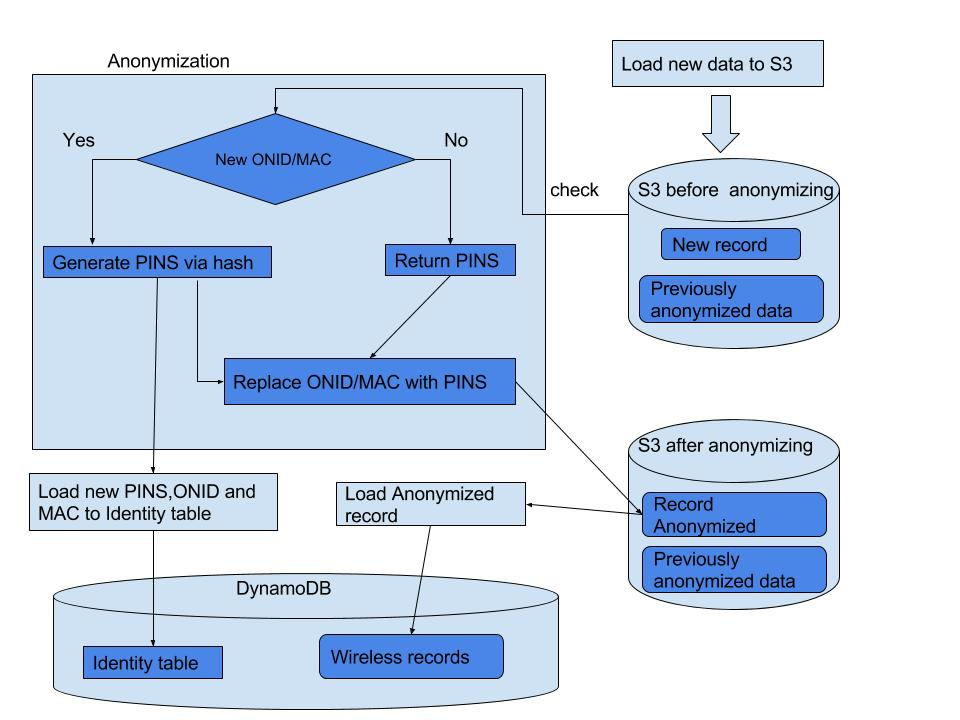
\includegraphics[width=17cm, height=12cm]{Pictures/workflow.jpg}
    \centering
    \caption{\label{fig:2}The workflow of importing new record}
\end{figure}

\noindent The workflow of the visualization starts from S3. After the DynamoDB table results have been stored back into S3, the data will be stored as CSV files in S3. These CSV files are important to the QuickSight because it requires the CSV files to generate the data set on the QuickSight console. After the data set have been created on the QuickSight console, the visualization will be easily generated. The figure \ref{fig:3} is the workflow of creating visualization on QuickSight.  

\begin{figure}[H]
	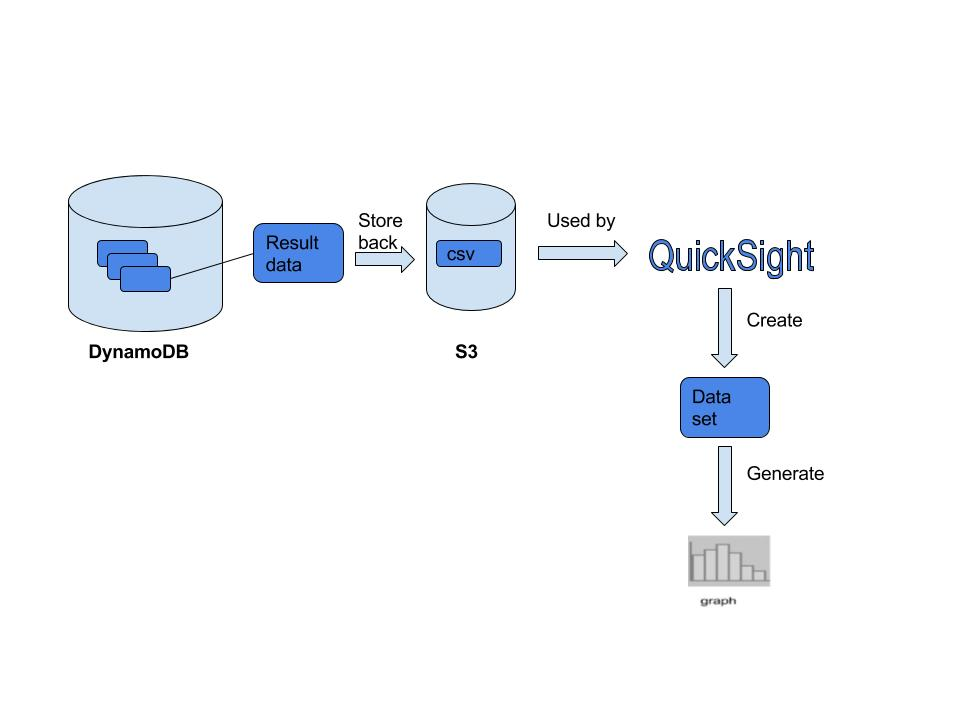
\includegraphics[width=17cm, height=10cm]{Pictures/QuickSight_workflow.jpg}
    \centering
    \caption{\label{fig:3}The workflow of creating visualization on QuickSight}
\end{figure}


\subsection{Operating instructions}
The project is working on the Amazon Web services, so it requires you must have a AWS account and this account has permission to access our project.\\

\noindent Load data from S3 into DynamoDB:
\begin{itemize}
	\item Connecting into the EC2 instance, run the python file \texttt{create.py} for creating table
    \item After creating tables, run the \texttt{import.py} for loading data login in the DynamoDB
    \item The command you need to type is \texttt{python import.py [input bucket name] [input file name] [output bucket name]}. The input bucket is the path of input file, and output bucket is the path of anoymized record.
    \item Check the result on the console Stop the EC2 instance on EC2 console
\end{itemize}

\noindent Save the result back to the S3:
\begin{itemize}
	\item Anonymized record have been created after run the import.py 
    \item This record is stored in a certain bucket
\end{itemize}

\noindent Create visualization on the QuickSight
\begin{itemize}
	\item Open the QuickSight console on AWS and Click New analysis button
    \item Choose New data set and click upload a file and choose the csv file which export from the "Records" table
    \item Using the data set and select the conlumn which need to evalaute
    \item Select the rows that need to evaluate and choose the visual types
    \item The visual will be created on right side    
\end{itemize}




    \newpage
    \section{The Approach to Learn New Technology}
	\subsection{Useful Websites}
    \noindent As for this project, The first helpful website is the Amazon Web Services introduction page. From this website, we learned the general steps for big data analysis. Another helpful website we find is the Boto3 Document, Boto3 is the Python SDK for Amazon Web Services. In this project, we are using the file system s3 to store the sample data and the DynamoDB for storing the processed data. The QuickSight will be using for doing the analysis. In general, the project will start with parsing sample data from S3. After that, the sample data will be processed and store into the DynamoDB. When we start coding, we use Python to load sample data from S3 the data into DynamoDB. Therefore, the Boto3 website helps us figure out how to load the sample data from S3 into DynamoDB by Python. 
    
    \subsection{Helpful People}
    \noindent The first helpful people on campus is our client David. He helps us on writing document. He gives useful feedback to us. So we can revise the document based on these feedback. The data analyst is also helpful. She helps us about permission for using the tool on AWS. Finally, our instructors and TA are very helpful. If we have problem with our project, we will ask them for help.

    \newpage
    i\section{Personal Statement}
	\subsection{Zhi Jiang}
In the past three terms, I learned a lot of things from this project. From a technical point perspective, I learned and understood some basic workflow and framework of big data. I still learned some valuable tools of cloud computing. In our project, we mainly used Amazon Web Services. This cloud platform provides many useful services to complete all kinds of operation for big data. For example, S3 is used to store all original data as a data storage; DynamoDB is a kind of NoSQL database; EC2 is a virtual machine to connect other services and operate data on them. Moreover, according to this project, I learned the advantage of cloud computing on big data. For instance, cloud computing platform can avoid large capital expenditure on upgrades and hardware. On the other hand, it can also improve cost efficiency by more closely matching your cost pattern to your demand pattern. The purpose of the client setting up this project is he would like to compare the cost of cloud platform and local hardware. On the other hand, most cloud providers are extremely reliable in providing their services such as AWS. The security of data and project maintenance can be guaranteed significantly.\\ 

\noindent The most thing I did in project work is research. In our project, we must use several services on AWS. I have never used them before, so I started to do research for those services. I read developer guide and learned their basic operation method hence doing research is a very helpful point in project work. In fact, a programmer will always face problems he or she has never seen, so the research is the best approach to solving it. Moreover, I am glad that I had carefully considered the alternative solution. For some reasons, I had to give up the prior solution in our original plan and chose the alternative solution. Eventually, we still completed my portion by this alternative solution. In the whole developing process, the accident may occur at any time. A good alternative can help developer deal with emergencies and ensure that processes are running smoothly.\\

\noindent I still learned many things from project management. I believe that the schedule should be the most important component in the project management. As we know, there are many uncontrollable factors in the development process such as new requirements. If you have an unreasonable and chaotic schedule,  any uncontrollable factors will make the influence on your development. On the contrary, the perfect plan can let you know what you did, what you should do right now, and what you left. You can understand the status of your project.\\ 

\noindent Teamwork is a necessary basis for success. By getting along with my teammates in these three terms, I found many benefits from collaboration. First of all, teamwork can increase the development efficiency, but the precondition is every member of this team should do their duty. If someone is lazy on the team, it will affect the performance of the entire team. Secondly, teamwork can more efficiently produce the best idea. A team comes up a more effective solution than one person dealing with on the same problem because each member has different knowledge and perspective. Meanwhile, I still learned that it was important to respect ideas of everyone because members have different habits and work styles. When we have different opinions with each other, the most appropriate way is to calmly discuss rather than quarrel. Thirdly, I feel I can learn more knowledge in teamwork because everyone has some skills that you don’t know such as programming language or an editing tool.\\

\noindent If I could do it all over, I believe user interface should be a good choice for this project. After visualization of analysis, the user interface can show the results to students. On the other hand, students are probably able to enter their person information to know their data in the campus. 
    \subsection{Zhaoheng Wang}
    	 \noindent The technical information I learned is the process of big data analysis on Amazon Web Services. The project for my group is to deal with the big data on Amazon Web Services. It is brand-new project for me. It is difficult to figure out how to start this project without any background knowledge. Fortunately, the homepage of Amazon web Service gives the general steps about how to deal with the big data on Amazon Web Services. In general, the big data will be generated from multiple sources and the data file might be unreadable. Therefore, the first step is called parse data. The purpose of this step is to format the data file and make it readable. After that, the parsed data needs to store and organize the storage place such as database. After the data has been organized, the visualization graph for the data will be created for analyzing.This is the technical information I learned from the project. \\
         
         \noindent The non-technical information and project work I learned is how to figure out a brand-new question. I believe it is impossible to solve every problem in the future work just based on the current knowledge I have. Therefore, the steps for solving a brand-new question will be a very important skill to have. In this project, I started with discussing with client. After discussion, I summarized the purpose and requirements for this project. Then, I started to search keywords such as AWS, big data, analysis and many others for this topic. According to searching information, I narrowed down the requirements and designed the general workflow for the whole project. After that, I discussed the project with my teammates and client to ensure that I was going the right direction. Personally, I think this skill is one of the most important skill I learned from this project.\\
         
         \noindent As for the project management and team working, I have learned that good communication will make team work more efficient. Through good communication, I work with my group better. For example, one of my teammates has experience working on big data analysis. When I had some question about the project, I asked his advice. Another skill I learned from team is to manage time and make the schedule for the project. As for my group, our personal schedule conflicted with each other most of time. Because of this, we made the group schedule for the project and this schedule helped us to finish the requirements on time.\\
         
         \noindent If I could do it all over, I would like to research more information about the project such as workflow and tools because it is very helpful to have more background knowledge before starting a project. Without any background knowledge, I spent more time on searching than I would have liked. Take my project as an example, the project my group worked on is to deal with the big data on the Amazon web service. At first, I had no idea about how to start the project. Therefore, I searched online about the big data analysis. However, there are many ways to do that so it is hard to decide which is the best way for dealing with the big data. Besides, I was not familiar with Amazon web service. Thus, I could only guess the step before starting this project. Because of this, the process for asking the permission for using the tool was complicated.\\
         
    \subsection{Isaac Chan}
\noindent I learned a bit more about different databases. I was previously aware of relational databases, specifically the more widely known AWS offering, Redshift. NoSQL with DynamoDB was new to me. However, I found that DynamoDB seemed to just a lazier version of Redshift because there was no upfront schema preparation, which might cause problems further on. Most of the other things, including workflow design, AWS utilities, I was already familiar with. \\

\noindent I think the most valuable non-technical information I learned was to constantly communicate with a client. I'm not sure if it was the balance of other classes or what, but during winter term, our communication with our client slipped a lot. We only met once or twice the entire term and he probably had no idea how we were progressing with his project. \\

\noindent In this project, it was very important to communicate with my group. We met a lot and were in constant communication, which helped us deliver on time and keep the schedule moving. I found it very helpful to develop a rough schedule and divide tasks early on. This meant that each of us was accountable for a portion and we progressed at a satisfactory rate. \\

\noindent If I could do it over again, I think I would have finished the project earlier on. The project itself was not very complex, but I felt like we were tied down by the structure of the class and how we were "supposed" to progress with it. Because of this, the project work was stretched out over winter and part of spring term, and it felt like we weren't doing a lot. \\
    
\end{document}
